\documentclass[12pt]{article}
\usepackage{tcolorbox}
\usepackage{graphicx, amsmath, amsthm, amsfonts, amssymb, indentfirst, enumitem, esint, verbatim, mathtools, fancyhdr, comment, wasysym, mathrsfs, stmaryrd, boxedminipage}
\usepackage{listings}
\usepackage{xcolor}
\usepackage{hyperref}
\usepackage{float}
\usepackage{chngcntr}
\usepackage[nameinlink,capitalise]{cleveref}

\crefname{figure}{figure}{Figure}   
\Crefname{figure}{Figure}{Figure}   

\hypersetup{
    colorlinks,
    citecolor=black,
    filecolor=black,
    linkcolor=black,
    urlcolor=black
}

\lstset{
    language=C,
    basicstyle=\ttfamily,
    keywordstyle=\color{blue}\bfseries,
    commentstyle=\color{gray},
    stringstyle=\color{red},
    identifierstyle=\color{black},
    xleftmargin=\parindent,
    showstringspaces=false, % Don't show spaces in strings
    morecomment=[l]{//} % Define line comments
}

\counterwithin{figure}{section}

\setlength{\leftmargini}{0.25in}
\setlength{\leftmarginii}{0.25in}
\setlength{\leftmarginiii}{0.25in}

\setlength{\parindent}{0pt}
\setlength{\parskip}{10pt}
\setlist{topsep=0pt,leftmargin=*}

\pagestyle{fancy}

\lhead{Joshua Nichols}
\rhead{18-213 Notes}

\author{Joshua Nichols}
\date{Summer 2024}
\title{18-213 Notes}

\begin{document}

\maketitle

\tableofcontents

\pagebreak
\section{Representing Data}

\pagebreak
\section{Assembly}

\pagebreak
\section{Memory Hierarchy}

\pagebreak
\section{Virtual Memory}

Processes in a CPU share memory between the various components in a computer - CPU caches, RAM, storage. To make memory management more efficient with fewer errors, modern systems provide an abstraction known as \textit{virtual memory}. Virtual memory presents main memory as a single contingous block which provides three main capibilities:

\begin{enumerate}
    \item It uses main memory efficiently by treating it as a cache for an address space on the disk, keeping only the active areas in main memory and transferring data back and forth between memory and disk as needed.
    \item It simplifies memory management by providing each process with a uniform address space.
    \item It protects the address space of each process from corruption by other processes.
\end{enumerate}

Virtual memory is one of the great ideas in computer systems, as it works automatically without any work required from the programmer. Although it works well behind the scenes, there are still several reasons for programmers to understand how virtual memory works:

\begin{itemize}
    \item \textit{Virtual memory is central}. Virtual memory defines all levels of computer systems, and influences the design of hardware exceptions, asemblers, linkers, loaders, shared objects, files, and processes. Understanding virtual memory will help you better understand how systems work in general.
    \item \textit{Virtual memory is powerful}. Virtual memory allows applications to create and destroy chunks of memory, map chunks of memory to portions of disk files, and share memory with other processes. For example, it's possible to modify the contents of a disk file by reading and writing memory locations, or to load the contents of a file into memory without doing any explicit copying.
    \item \textit{Virtual memory is dangerous}. Applications interact with virtual memory every time they reference a variable, dereference a pointer, or make a call to dynamic allocation packages such as \lstinline{malloc}. If virtual memory is used improperly it can lead to memory-related bugs.
\end{itemize}

\subsection{Physical and Virtual Addressing}

The main memory of a computer is organized as an array of $M$ contingous byte-sized cells. Each byte has a \textit{physical address} (PA). The first byte has an address of $0$, the next byte has an address of $1$, etc. Given this simple organizanization, it makes sense for a CPU to access memory using physical addresses, an approach known as \textit{physical addressing}.

\Cref{fig:41} demonstrates an example in the context of a load instruction that reads the $4$-byte word starting at physical address $4$. When the CPU executes the load instruction, it generates an effective physical address and passes it to the main memory over the memory bus. The main memory fetches the $4$-byte word starting at physical address $4$ and returns it to the CPU, which stores it in a register.

\begin{figure}[H]
    \centering
    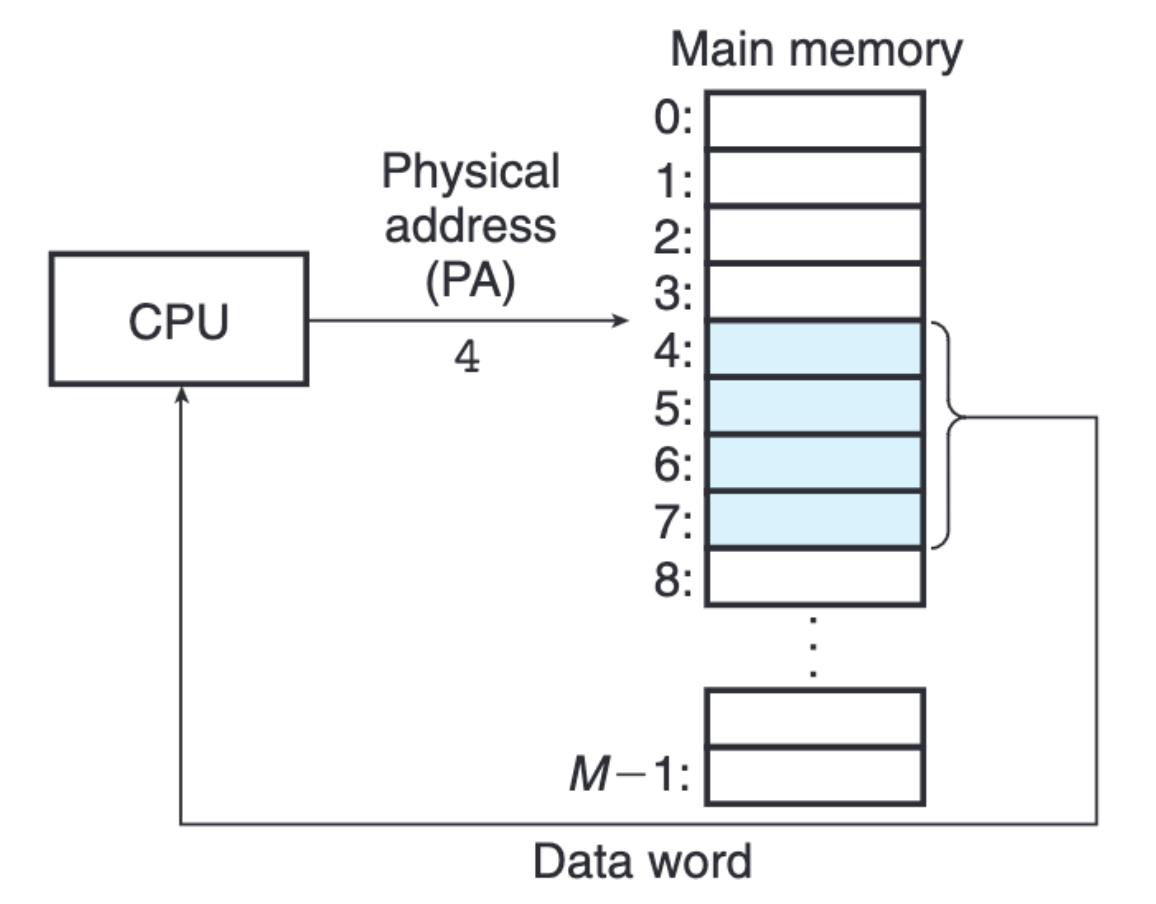
\includegraphics[width=0.75\textwidth]{graphics/Figure 4.1.png}
    \caption{A system that uses physical addressing}
    \label{fig:41}
\end{figure}

In contrast, most modern processors use a form of addressing known as \textit{virtual addresing}, shown in \Cref{fig:42}. With virtual addressing, the CPU accesses main memory by generating a \textit{virtual address} (VA), which is converted to the appropiate physical address before being sent to main memory. The task of converting a virtual address to a physical one is known as \textit{address translation}.

\begin{figure}[H]
    \centering
    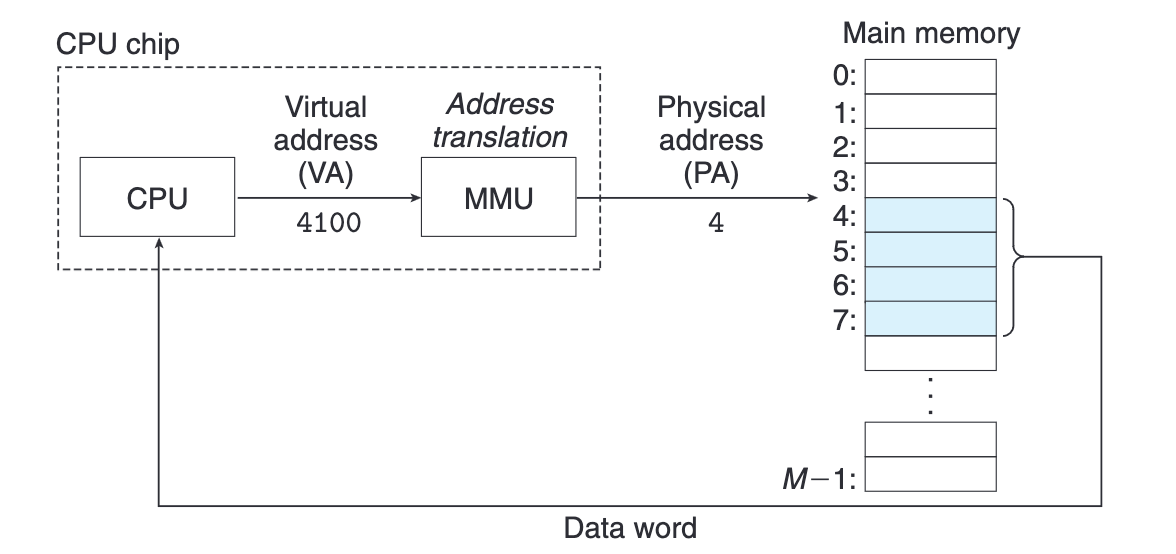
\includegraphics[width=0.75\textwidth]{graphics/Figure 4.2.png}
    \caption{A system that uses virtual addressing}
    \label{fig:42}
\end{figure}

Like exception handling, address translation requires close cooperation between the CPU and the operating system. Dedicated hardware on the CPU chip called the \textit{memory management unit} (MMU) translates virtual addresses on the fly, using a lookup table stored in main memory whose contents are managed by the operating system.

\subsection{Address Spaces}

An \textit{address space} is an ordered set of nonnegative integer addresses:
\[ \{0,1,2,\ldots\} \]
If the integers in the address space are consecutive, then we say it is a \textit{linear address space}. To simplify our discussion, we will always assume linear address space. In a system with virtual memory, the CPU generates virtual addresses from an address space of $N=2^n$ addresses called the \textit{virtual address space}.
\[ \{0,1,2,\ldots N-1\} \]
The size of an address space is characterized by the number of bits that are needed to represent the largest address. For example, a virtual address space with $N=2^n$ addresses is called an $n$-bit address space. Modern systems typically support $32$-bit or $64$-bit virtual address spaces.

A system also has a \textit{physical address space} that corresponds to $M$ bytes of physical memory in the system:
\[ \{0,1,2,\ldots,M-1\} \]
$M$ is not required to be a power of $2$, but to simplify the discussion, we will assume that $M=2^m$.

The concept of an address space is important because it makes a clean distinction between data objects (bytes) and their attributes (addresses). Once we recognize this distinction, we can then generalize and allow each data object to have several independent addresses, each chosen from a different address space. This is the basic idea of virtual memory. Each byte of memory has a virtual address chosen from the virtual address space, and a physical address chosen from the physical address space.

\subsection{Virtual Memory as a Tool for Caching}

Virtual memory is organized as an array of $N$ contigous byte-size cells stored on disk. Each byte has a unique virtual address that serves as an index into the array. The contents of the array on disk are cached in main memory. 

As with any other cache in the memory hierarchy, the data on disk (lower level) is partitioned into blocks that serve as transfer units between the disk and main memory (upper level). VM systems handle this by partitioning the virtual memory into fixed-size blocks called \textit{virtual pages} (VPs). Each virtual space is $P=2^p$ bytes in size. Similarly, physical memory is partitioned into \textit{physical pages} (PPs), also $P$ bytes in size. Physical pages are also referred to as \textit{page frames}.

The set of virtual pages is partitioned into three disjoint subsets:
\begin{enumerate}
    \item \textit{Unallocated} - Pages that have not yet been allocated by the virtual memory system. Unallocated blocks do not have any data associated with them, and thus do not occupy any space on disk.
    \item \textit{Cached} - Allocated pages that are currently cached in physical memory.
    \item \textit{Uncached} - Allocated pages that are not cached in physical memory.
\end{enumerate}

\begin{figure}[H]
    \centering
    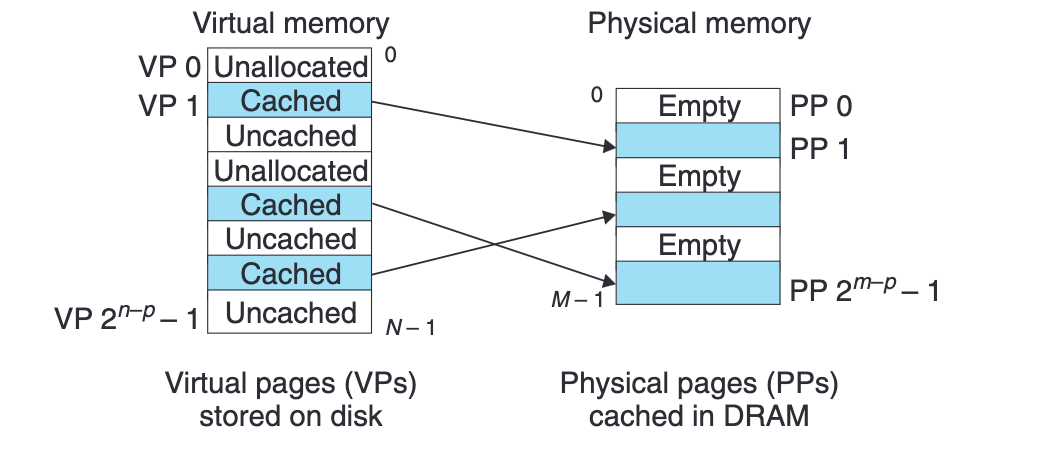
\includegraphics[width=0.75\textwidth]{graphics/Figure 4.3.png}
    \caption{How a VM system uses main memory as a cache}
    \label{fig:43}
\end{figure}

\subsubsection*{DRAM Cache Organization}



\subsubsection*{Page Tables}

\begin{figure}[H]
    \centering
    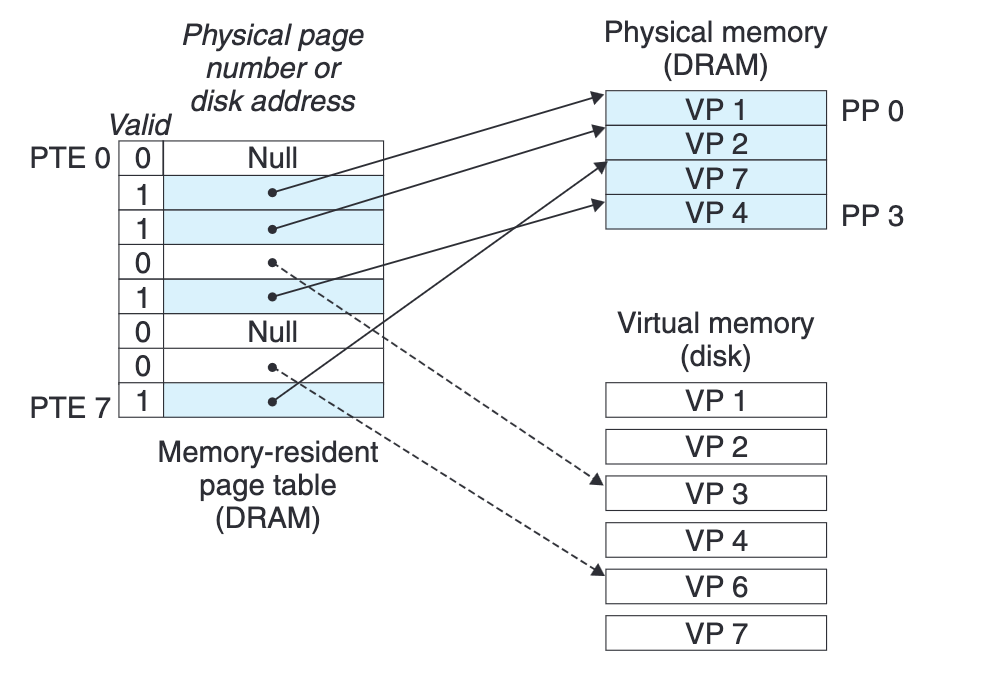
\includegraphics[width=0.75\textwidth]{graphics/Figure 4.4.png}
    \caption{Page table}
    \label{fig:44}
\end{figure}

\subsubsection*{Page Hits}



\subsubsection*{Page Faults}

In discussions of virtual memory, a DRAM cache miss is known as a \textit{page fault}. 

Taking an example, we begin with the state of memory in \Cref{fig:45}:

\begin{figure}[H]
    \centering
    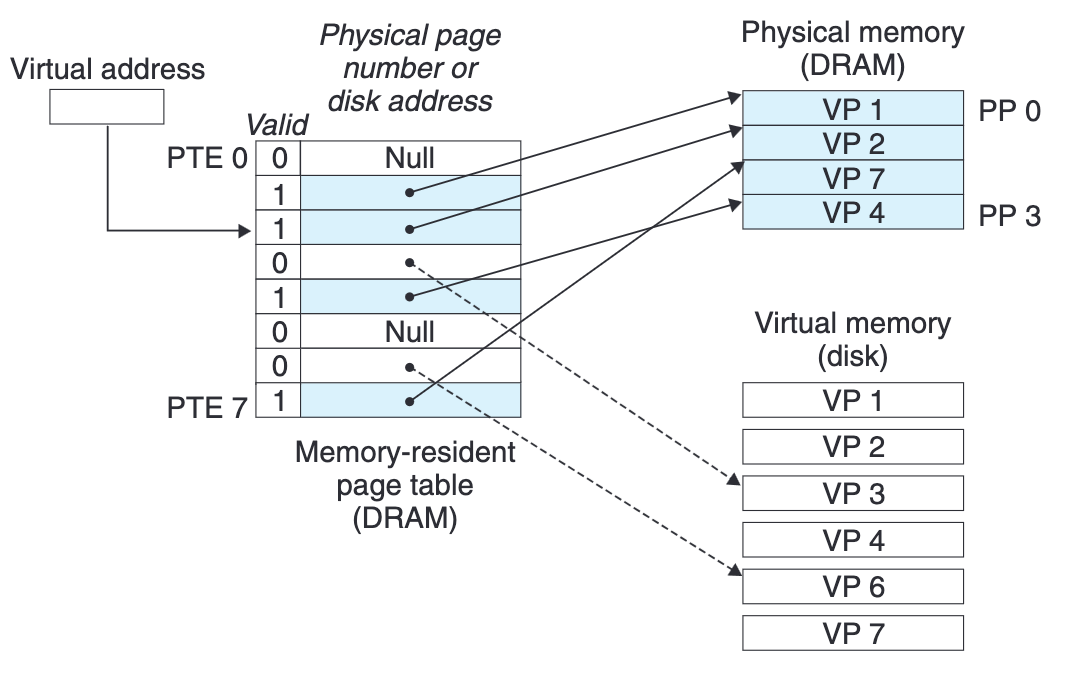
\includegraphics[width=0.75\textwidth]{graphics/Figure 4.5.png}
    \caption{}
    \label{fig:45}
\end{figure}



\begin{figure}[H]
    \centering
    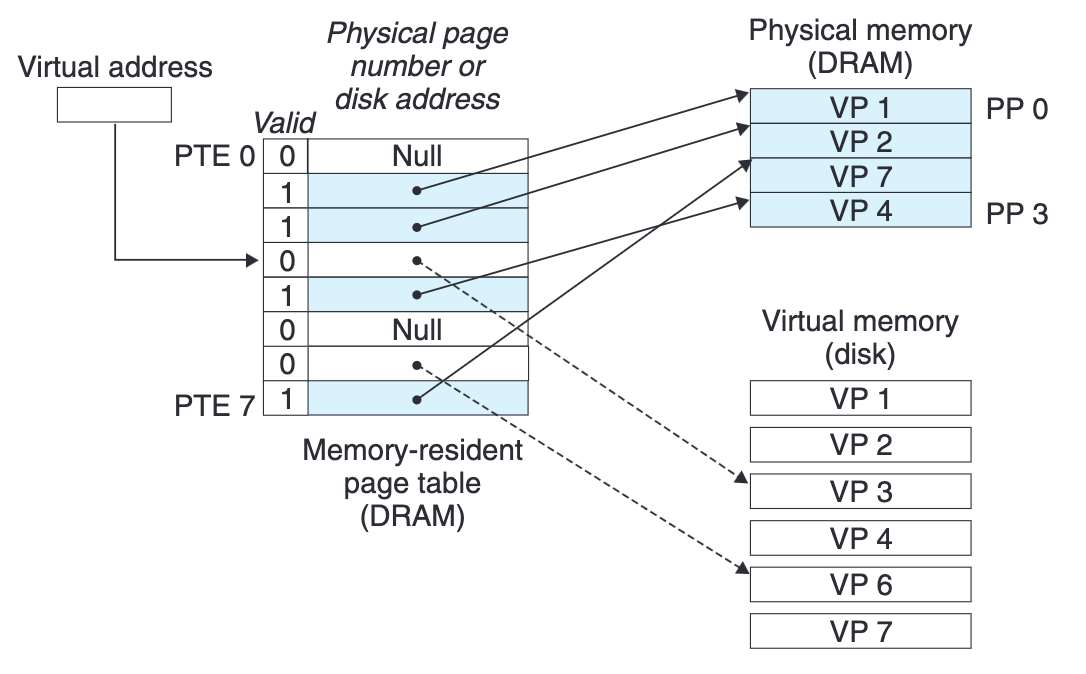
\includegraphics[width=0.75\textwidth]{graphics/Figure 4.6.png}
    \caption{VM page fault (before)}
    \label{fig:46}
\end{figure}

\begin{figure}[H]
    \centering
    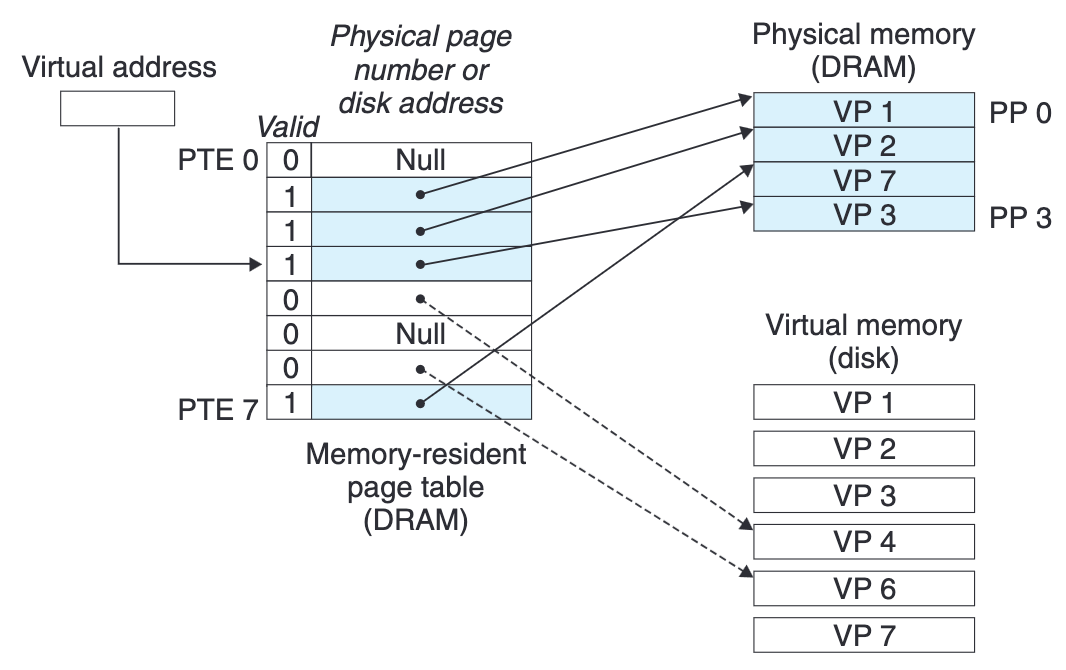
\includegraphics[width=0.75\textwidth]{graphics/Figure 4.7.png}
    \caption{VM page fault (after)}
    \label{fig:47}
\end{figure}

\subsubsection*{Allocating Pages}



\subsubsection*{Locality}


\end{document}